% !TEX TS-program = pdflatex
% !TEX encoding = UTF-8 Unicode

% This is a simple template for a LaTeX document using the "article" class.
% See "book", "report", "letter" for other types of document.
\documentclass[12pt]{article} % use larger type; default would be 10pt

%\documentclass{amsart}
\usepackage[utf8]{inputenc} % set input encoding (not needed with XeLaTeX)
\usepackage{hyperref}
\usepackage{listings}
\usepackage{movie15}
\usepackage{graphicx}

\hypersetup{
    colorlinks=true,
    linkcolor=blue,
    filecolor=magenta,      
    urlcolor=blue,
}

%%% Examples of Article customizations
% These packages are optional, depending whether you want the features they provide.
% See the LaTeX Companion or other references for full information.

%%% PAGE DIMENSIONS
\usepackage{geometry} % to change the page dimensions
\geometry{a4paper} % or letterpaper (US) or a5paper or....
% \geometry{margin=2in} % for example, change the margins to 2 inches all round
% \geometry{landscape} % set up the page for landscape
%   read geometry.pdf for detailed page layout information

\usepackage{graphicx} % support the \includegraphics command and options

% \usepackage[parfill]{parskip} % Activate to begin paragraphs with an empty line rather than an indent

%%% PACKAGES
\usepackage{booktabs} % for much better looking tables
\usepackage{array} % for better arrays (eg matrices) in maths
\usepackage{paralist} % very flexible & customisable lists (eg. enumerate/itemize, etc.)
\usepackage{verbatim} % adds environment for commenting out blocks of text & for better verbatim
\usepackage{subfig} % make it possible to include more than one captioned figure/table in a single float
% These packages are all incorporated in the memoir class to one degree or another...

%%% HEADERS & FOOTERS
\usepackage{fancyhdr} % This should be set AFTER setting up the page geometry
\pagestyle{fancy} % options: empty , plain , fancy
\renewcommand{\headrulewidth}{0pt} % customise the layout...
\lhead{}\chead{}\rhead{}
\lfoot{}\cfoot{\thepage}\rfoot{}

%%% SECTION TITLE APPEARANCE
\usepackage{sectsty}
\allsectionsfont{\sffamily\mdseries\upshape} % (See the fntguide.pdf for font help)
% (This matches ConTeXt defaults)

%%% ToC (table of contents) APPEARANCE
\usepackage[nottoc,notlof,notlot]{tocbibind} % Put the bibliography in the ToC
\usepackage[titles,subfigure]{tocloft} % Alter the style of the Table of Contents
\renewcommand{\cftsecfont}{\rmfamily\mdseries\upshape}
\renewcommand{\cftsecpagefont}{\rmfamily\mdseries\upshape} % No bold!

%%% END Article customizations

%%% The "real" document content comes below...

\title{EECS 233 HW6}
\author{Ben Pierce \\ \texttt{bgp12@case.edu}}
%\date{} % Activate to display a given date or no date (if empty),
         % otherwise the current date is printed 




%if anyone's reading this, any Latex tips/tricks would be greatly appreciated. 

\begin{document}
\maketitle
\title {GitHub: https://github.com/bp0017/CWRUEECS233/tree/master/HW6} 

\section{Question 1: Binary Tree Traversal}
\subsection{Pre-order}
Values: 9 3 2 1 6 5 4 7 8
\subsection{In-order}
Values: 1 2 3 4 5 6 7 8 9
\subsection{Post-order}
Values: 1 2 4 5 8 7 6 3 9

\section{Question 2: Insert and Remove}
a)\\
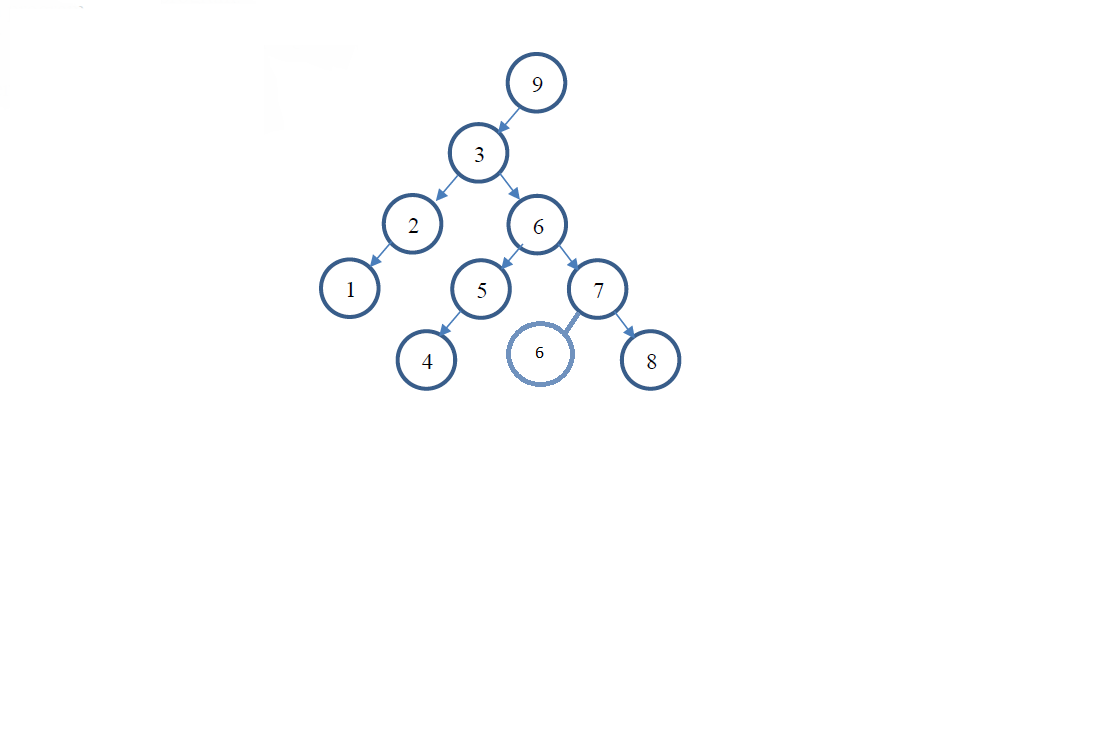
\includegraphics[scale = 0.5]{a.png}

b)\\
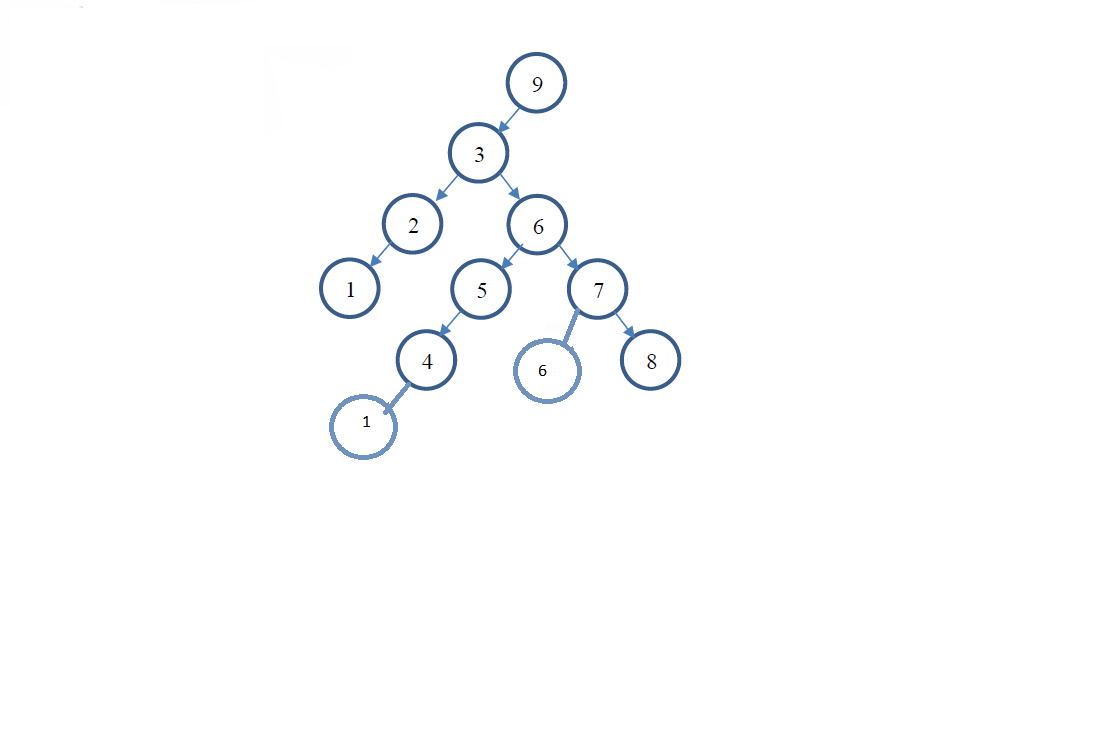
\includegraphics[scale = 0.5]{b.png}

c)\\
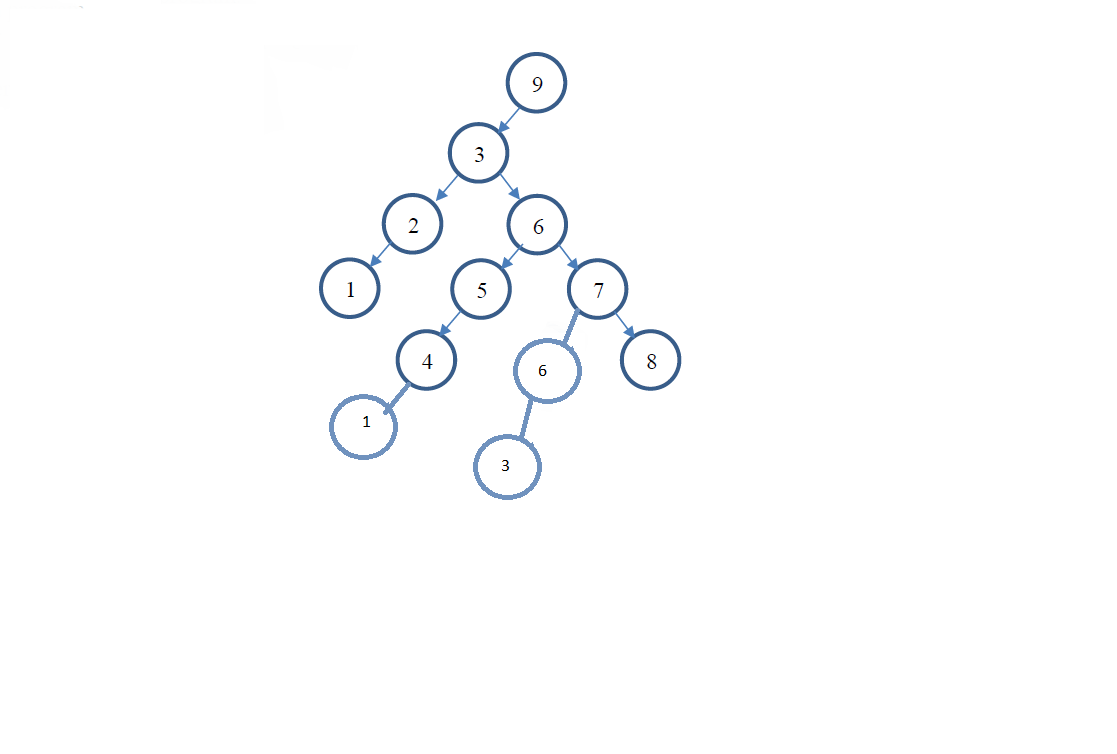
\includegraphics[scale = 0.5]{c.png}

d)\\
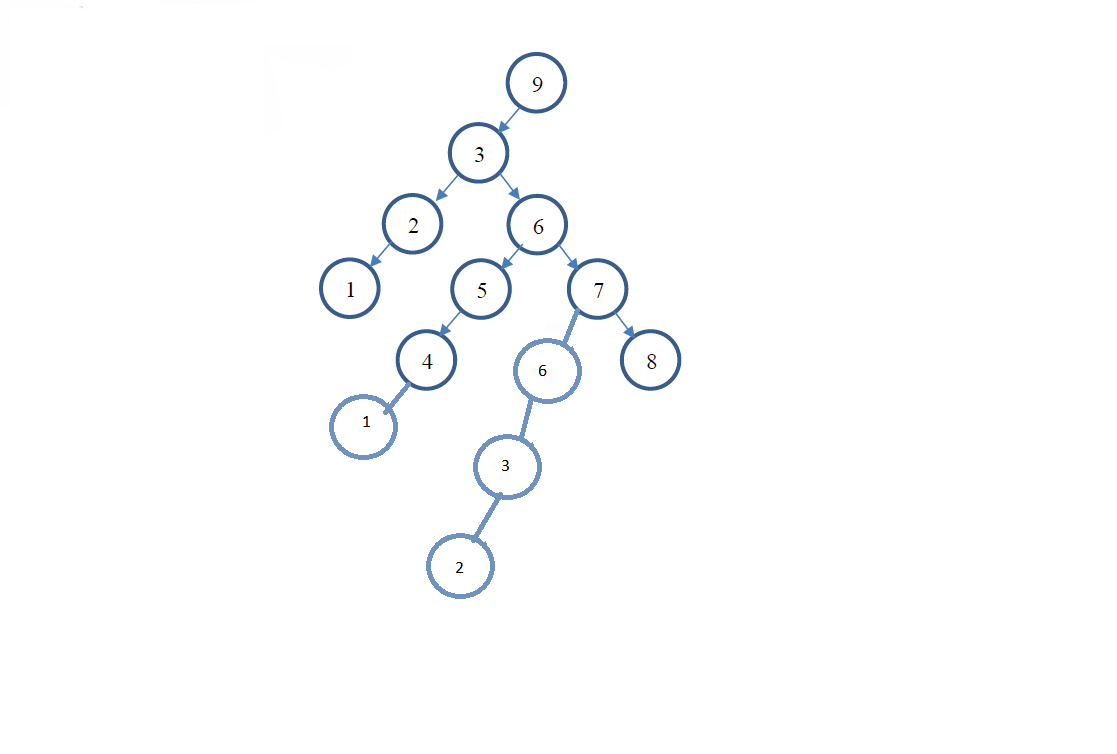
\includegraphics[scale = 0.5]{d.png}

e)\\
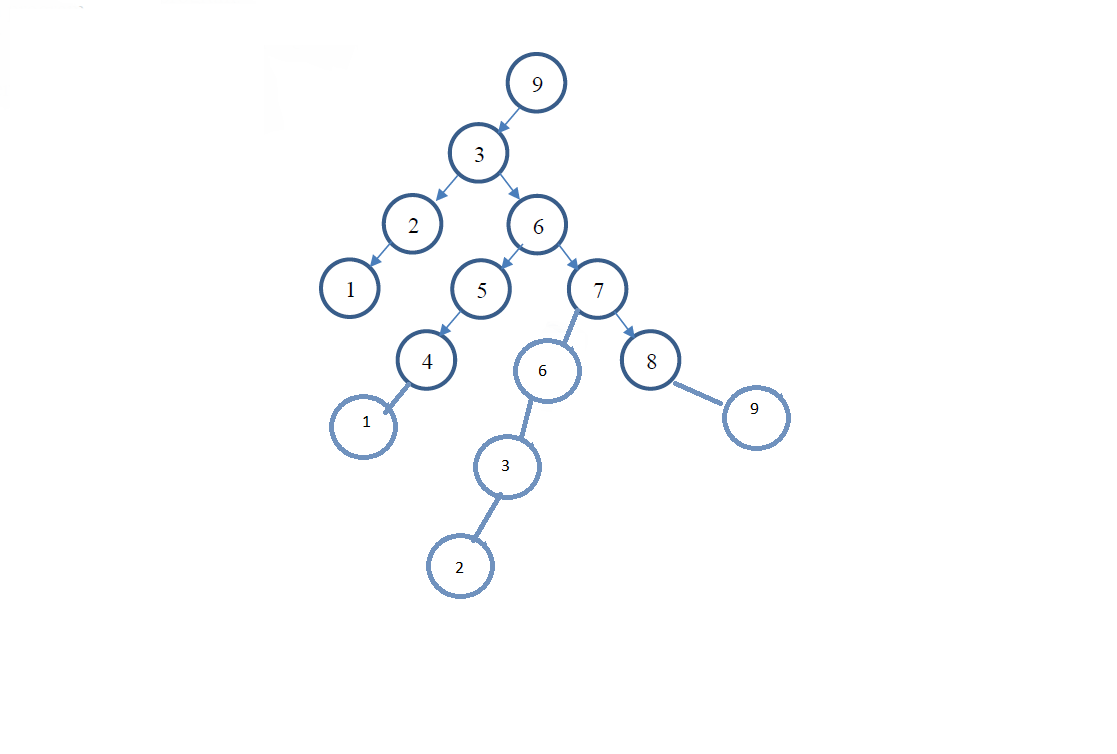
\includegraphics[scale = 0.5]{e.png}

f)\\
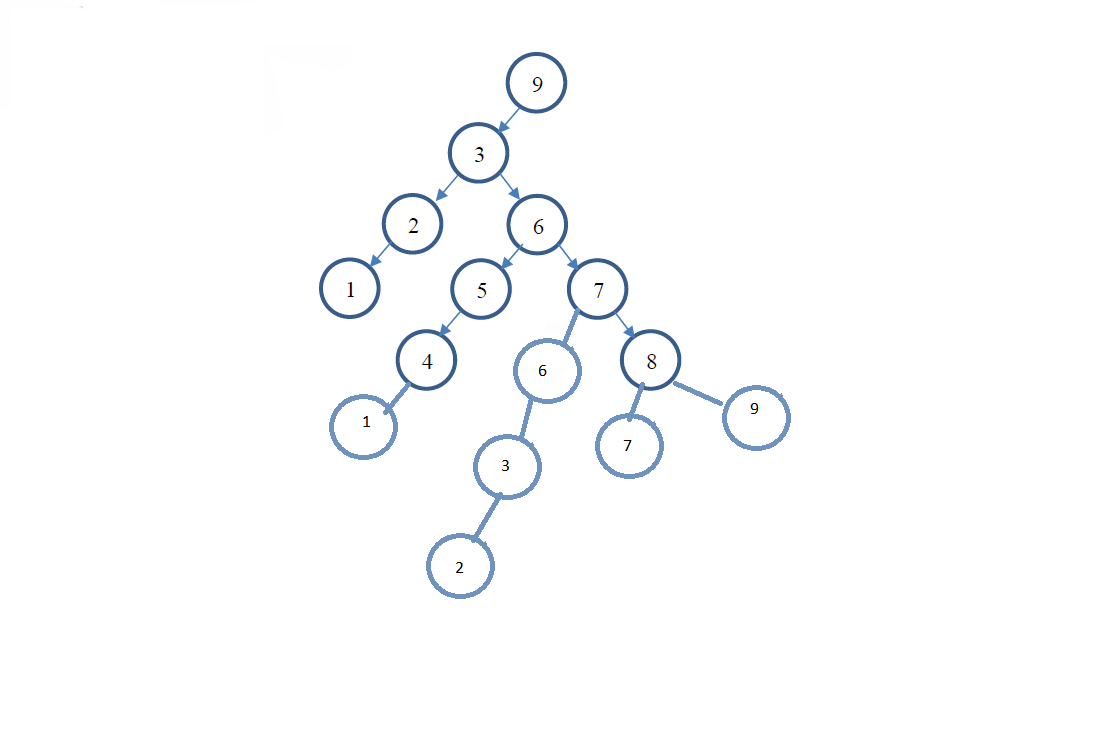
\includegraphics[scale = 0.5]{f.png}

g)\\
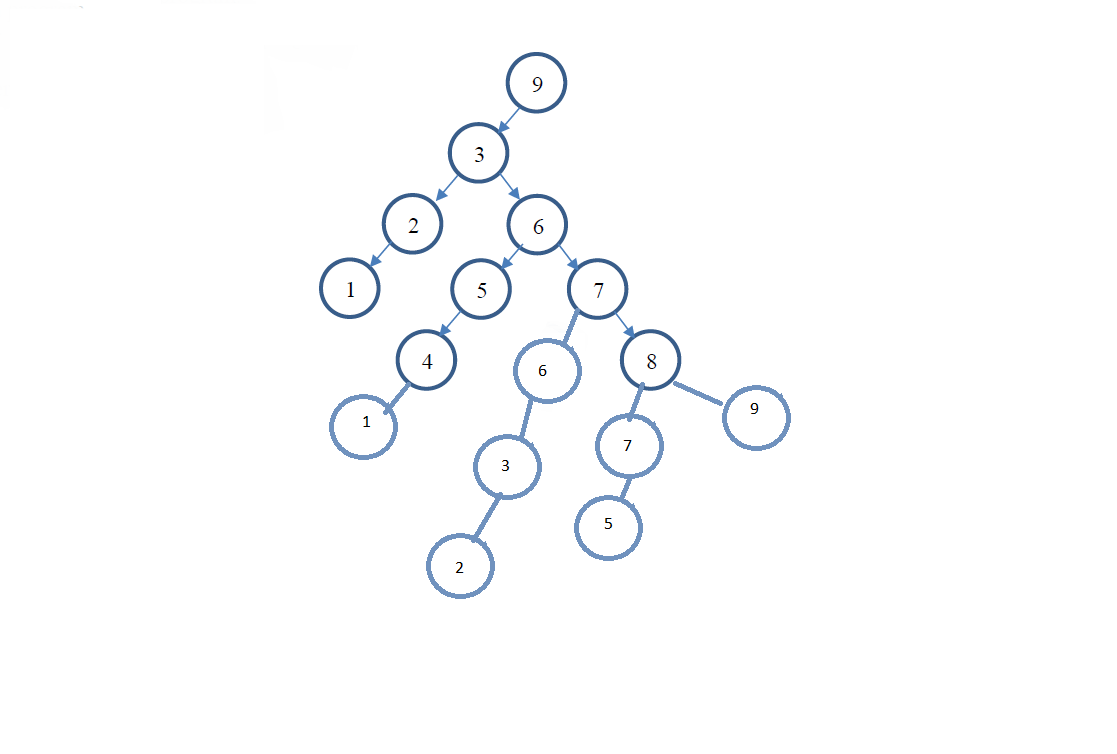
\includegraphics[scale = 0.5]{g.png}

h)\\
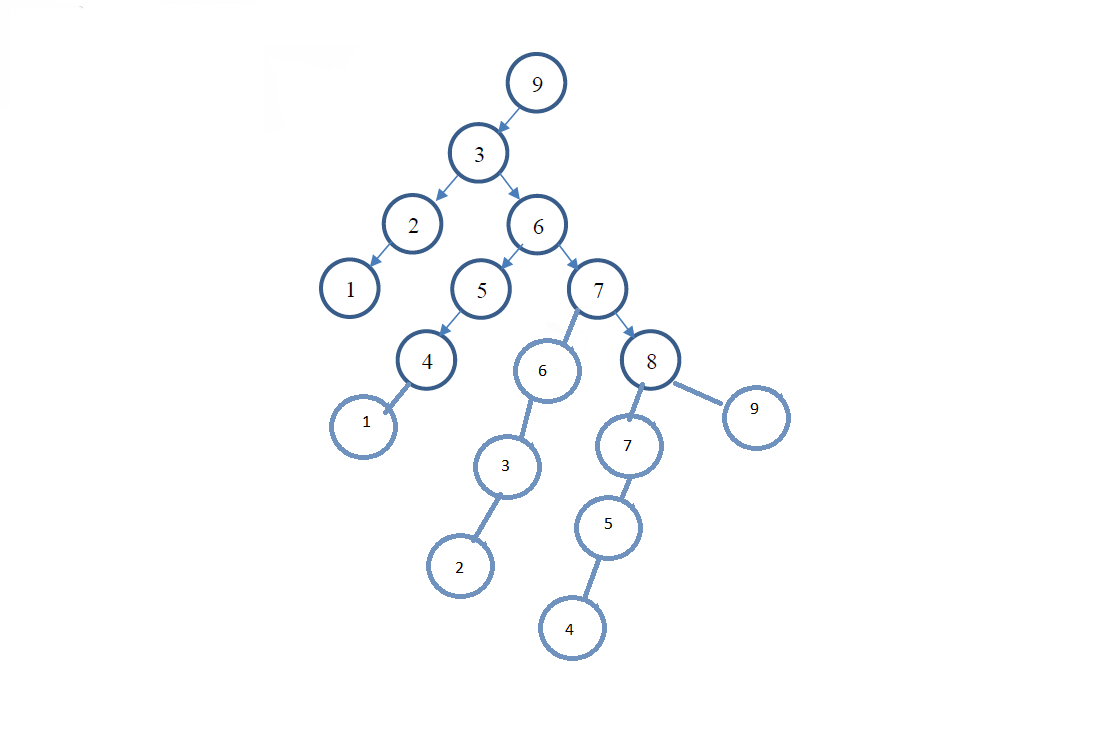
\includegraphics[scale = 0.5]{h.png}

i)\\
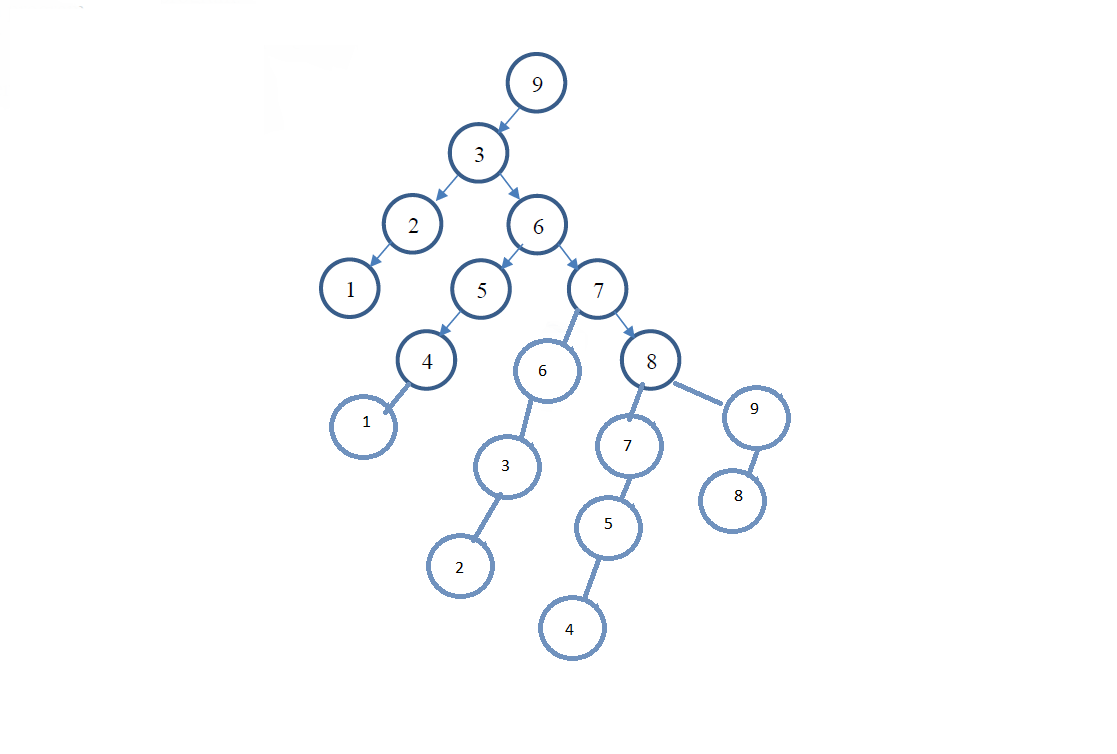
\includegraphics[scale = 0.5]{i.png}

j)\\
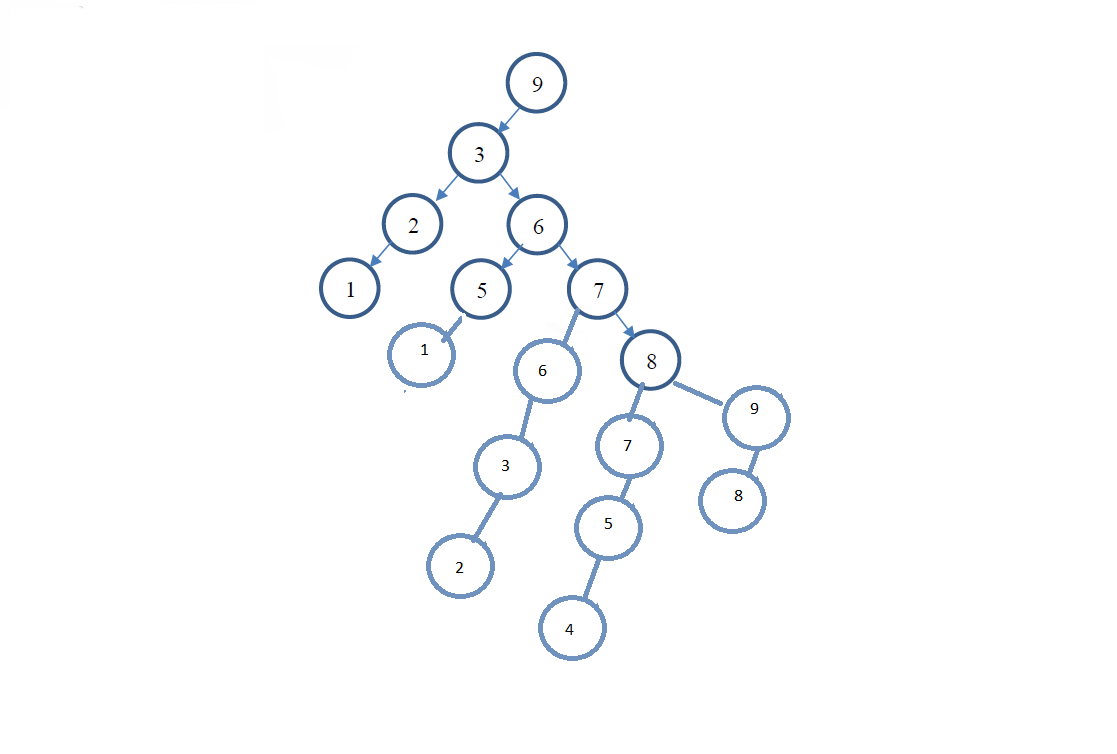
\includegraphics[scale = 0.5]{j.png}

k)\\
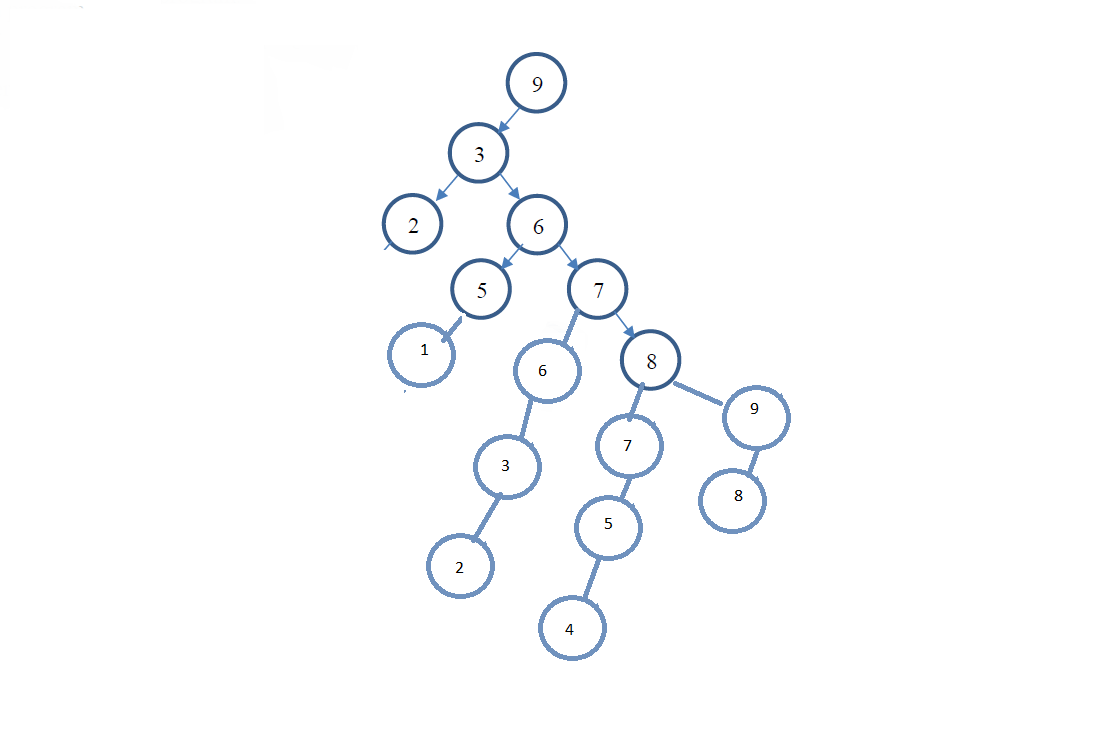
\includegraphics[scale = 0.5]{k.png}

l)\\
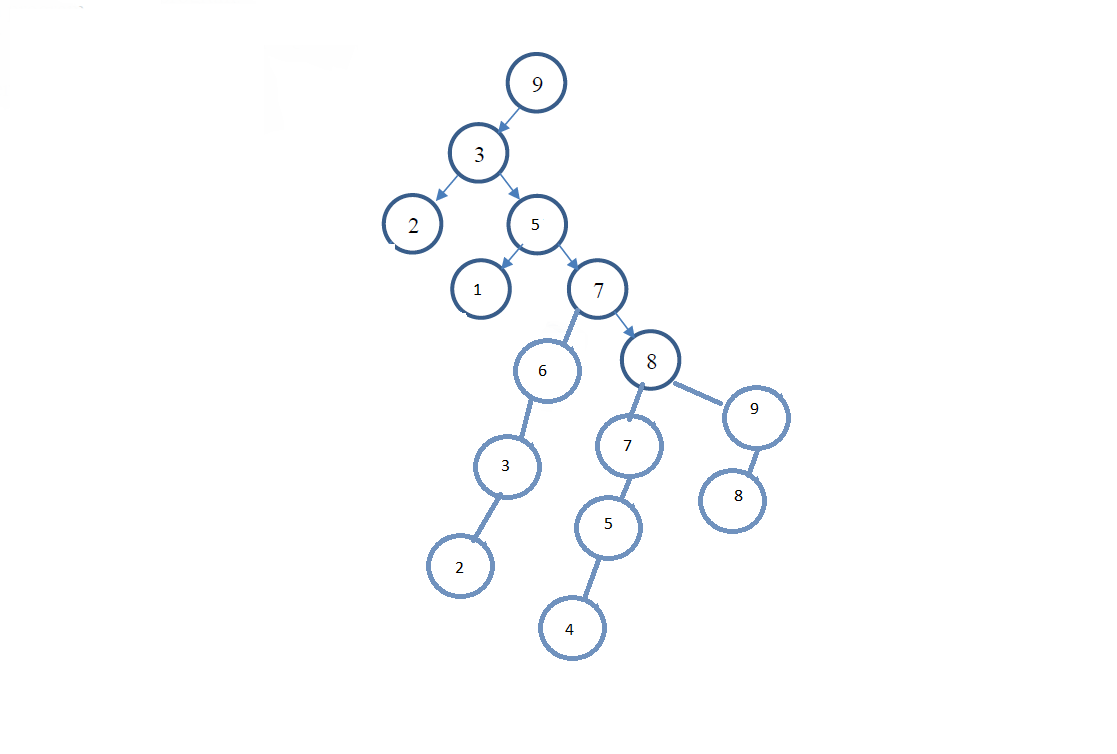
\includegraphics[scale = 0.5]{l.png}

\section{Question 3: Code Output}
\begin{lstlisting}
C:\Users\bp001\Documents\EECS223\HW6>java IntTreeBag2
Preorder Print method:
9
3
2
1
6
5
4
7
8
Inorder Print method:
1
2
3
4
5
6
7
8
9
Postorder Print method:
1
2
4
5
8
7
6
3
9
\end{lstlisting}


\end{document}